


\subsection{Αλγόριθμος Bresenham για ευθύγραμμο τμήμα}

Το $1965$ ο J.E. Bresenham παρουσίασε την πρώτη DDA μέθοδο (Digital Differential Analyzer) για το σχεδιασμό ευθύγραμμου τμήματος. Εκεί παρουσίαζε τη μορφή που έχει ο αλγόριθμός του για ευθύγραμμα τμήματα που ανήκουν στο πρώτο οκταμόριο. Δηλαδή που η γωνία που σχηματίζουν με τον οριζόντιο άξονα είναι από $0$ εώς $\ang{45}$. Καθώς και τις μετατροπές που χρειάζονται να γίνουν για να μπορούμε να σχεδιάσουμε ευθύγραμμα τμήματα κάθε κλίσης.


\begin{figure}[h!]
  \begin{center}
	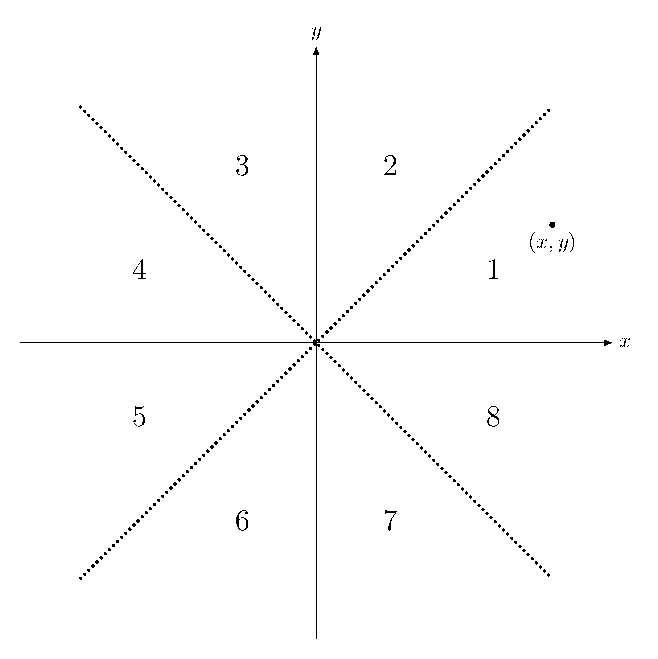
\includegraphics[scale=0.5]{Chapter1/Bresenham/octamoriums.pdf}
  \end{center}
  \caption{Τα οκταμόρια του επιπέδου}
\end{figure}


Προσδιορίζουμε το σχεδιασμό της ευθείας στο $1$ο οκταμόριο και στη συνέχεια με κατάλληλη τροποποίηση, που θα την περιγράψουμε παρακάτω, μπορούμε να επεκταθούμε και στα άλλα οκταμόρια.

΄Εστω ότι θέλουμε να σχεδιάσουμε ένα ευθύγραμμο τμήμα $\overline{P_1 P_2}$, για pixels τα οποία ανήκουν στο $1$ο οκταμόριο, έστω $P_1= (x_1, y_1), P_2= (x_2, y_2)$. 

Έστω ότι έχει φωτισθεί στην οθόνη το pixel $P_i (x_i , y_i)$.

\begin{figure}[h!]
  \begin{center}
	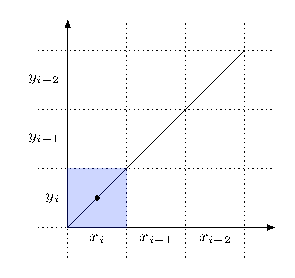
\includegraphics{Chapter1/Bresenham/bresenham-stepwise/bresenham-zero.pdf}
  \end{center}
  \caption{Σχεδιασμός ευθύγραμμου τμήματος μεταξύ των pixel στο $1$ο οκταμόριο}
\end{figure}





Δεδομένου ότι ο σχεδιασμός του ευθυγράμμου τμήματος συνίσταται στον επιλεκτικό φωτισμό διαδοχικών pixels ώστε αυτά να σχηματίζουν ευθύγραμμο τμήμα, θεωρούμε ότι αφού βρισκόμαστε στο 1ο οκταμόριο εάν ήδη είναι φωτισμένο το pixel $P_i(x_i , y_i)$ τα επόμενα δυνατά προς φωτισμό pixels θα είναι τα $P_{i+1}(x_{i+1} , y_i)$ ή $P_{i+1}(x_{i+1} , y_{i+1})$

Παρατηρούμε δηλαδή ότι οπωσδήποτε θα αυξηθεί κατά $1$ η συντεταγμένη x και η συντεταγμένη y ή θα παραμείνει ίδια ή θα αυξηθεί κι αυτή κατά $1$. Θα πρέπει, λοιπόν να καθορίσουμε μία μεταβλητή σφάλματος, η οποία ανάλογα να αποφαίνεται εάν θα αυξηθεί ή όχι η συντεταγμένη $y$.

\subsection{Δημιουργία μεταβλητής σφάλματος $\epsilon_i$}

Η εξίσωση μεταξύ των σημείων $(x_i,y_i)$ και $(x_{i + 1}, y)$ είναι  
%
\[
	y =sx_{i+1}+c, 
\]
όπου,
\begin{align*}
	s &= \cfrac{y-y_i}{x_i+1-x_i} = \cfrac{\Delta y}{\Delta x} \leq 1, \text{η κλίση της ευθέιας} \\
	c &= \cfrac{y_i x_{i+1} - y x_i}{x_{i+1}-x_i}
\end{align*}
%
%
Υπολογίζουμε τις αποστάσεις $d_1, d_2$ και της διαφορά τους $d_1-d_2$:

\begin{align*} 
	d_1 &= y-y_i = s(x_i+1)+c-y_i \\
	d_2 &= (y_i+1)-y = y_i+1- s(x_i+1)-c \\
	d_1-d_2 &= 2s(x_i+1) - 2y_i +2c-1
\end{align*}

\begin{figure}[hbt]
  \begin{center}
	  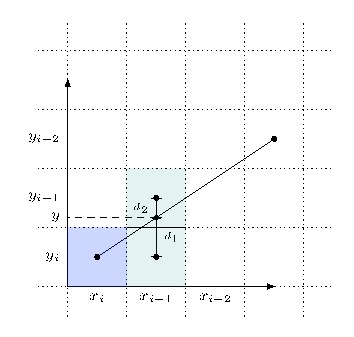
\includegraphics[]{Chapter1/Bresenham/bresenham-stepwise/bresenham-first-step.pdf}
  \end{center}
  \caption{}
\end{figure}



\begin{remark}
	 Ανάλογα με το πρόσημο της διαφοράς $d_1-d_2$ μπορούμε να επιλέξουμε το επόμενο προς φωτισμό pixel. 	
\end{remark}

Εάν ονομάσουμε μεταβλητή σφάλματος, $e_i$, την ποσότητα $e_i = \Delta x(d_1 − d_2)$ τότε θα έχουμε :

\begin{table}[h!]
\centering
\begin{tabular}{cc}
\toprule
$e_i$      & Επόμενο προς φωτισμό pixel \\
\midrule
$< 0$      & $(x_i+1, y_i)$ \\
$\geq 0$   & $(x_i+1, y_i+1)$ \\
\bottomrule
\end{tabular}
\caption{Πίνακας με κριτήριο προσδορισμού επόμενο προς φωτισμό pixel.}
\label{tab:next_pixel}
\end{table}


\subsection{Προσπάθεια δημιουργίας αναδρομικού τύπου}

Σε κάθε βήμα σχεδιασμού της ευθείας θα είναι καλό να μπορούμε να υπολογίζουμε την καινούρια μεταβλητή σφάλματος συναρτήσει της προηγούμνηες, γι' αυτό προσπαθούμε να δημιουργήσουμε έναν αναγωγικό τύπο. Ισχύει ότι:

\begin{equation*}
	e_i = \Delta x(d_1-d_2).	
\end{equation*}

%
Καθώς,
%
\begin{equation*}
	  \left.\begin{aligned}
	  s &= \cfrac{\Delta y}{\Delta x}	\\
	  d_1 &= y-y_i = s(x_i+1)+c-y_i\\
	  d_2 &= (y_i+1)-y = y_i+1- s(x_i+1)-c	
	\end{aligned}\right\} \Rightarrow e_i = \cfrac{\Delta y}{s} (2s(x_i+1)-2y_i+2c-1)
\end{equation*}
 Αφού όμως, $\cfrac{\Delta y}{s} = \Delta x$, συνολικά έχουμε ότι:
 %
\begin{align*}
	e_i = 2\Delta y(x_i+1) - 2\Delta xy_i + \Delta x(2c − 1) 
		= 2\Delta yx_i - 2\Delta xy_i +c', \quad c' = 2\Delta y + \Delta x(2c − 1) \tag{1}
 	\label{eq:1}
\end{align*}
%
Λόγω της \eqref{eq:1}, για το $e_{i+1}$ θα ισχύει: 
%
\begin{equation*}
	e_{i+1} = 2\Delta yx_{i+1} − 2\Delta xy_{i+1} + c'.
\end{equation*}
%
Τελικά,
%
\begin{align*}
	e_{i+1}-e_i &= 2\Delta yx_{i+1} − 2\Delta xy_{i+1} + c'- 2\Delta yx_i + 2\Delta xy_i -c' = \\\
				&= 2\Delta y (x_{i+1}-x_i)-2\Delta x(y_{i+1}-y_i)		
\end{align*}
%
Για $i=1$, $(x_1,y_1) \equiv (0,0)$. Οπότε, αξιοποιώντας την \eqref{eq:1}, λαμβάνουμε:

\begin{itemize}
	\item $c = \cfrac{y_i x_{i+1} - y x_i}{x_{i+1}-x_i} 
  =	\cfrac{y_1 \cdot(x_1+1) - y \cdot x_1}{x_1+1-x_1}
  = 0 \cdot(0+1) - y \cdot 0
  = 0 $
	\item $e_1 = 2\Delta y \cdot 0 - 2\Delta x\cdot 0 +2\Delta y + \Delta x (2c-1) 
	= 2\Delta y + 2\Delta x \cdot c - \Delta x \overset{c=0}{=} 2\Delta y - \Delta x$
\end{itemize}
%
Προκύπτει, λοιπόν, ότι:
%
\begin{table}[h!]
\centering
\begin{tabular}{l c}
\toprule
\multicolumn{1}{c}{$e_1$} & \multicolumn{1}{c}{Επόμενη μεταβλητή σφάλματος $e_2$} \\
\midrule
$< 0 \to (x_i+1, y_i)$       & $e_1 + 2\Delta y$                  \\
$\geq 0 \to (x_i+1, y_i+1)$  & $e_1 + 2\Delta y - 2\Delta x$      \\
\bottomrule
\end{tabular}
\caption{Πίνακας με τις συνθήκες και τις μεταβλητές σφάλματος.}
\label{tab:error_conditions}
\end{table}


\begin{figure}[h!]
\begin{center}
\begin{minipage}[b]{0.48\textwidth} % Top-left image
%    \centering
    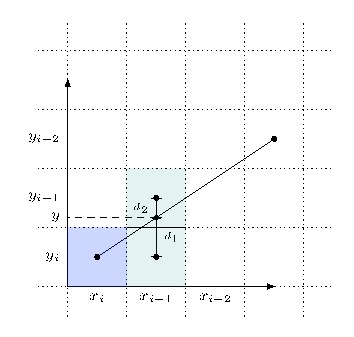
\includegraphics[width=\textwidth]{Chapter1/Bresenham/bresenham-stepwise/bresenham-first-step.pdf}
    \captionof{figure}{Top-Left Image}
\end{minipage}%
\hfill
\begin{minipage}[b]{0.48\textwidth} % Top-right image
%    \centering
    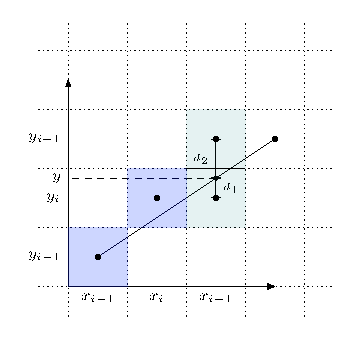
\includegraphics[width=\textwidth]{Chapter1/Bresenham/bresenham-stepwise/bresenham-second-step.pdf}
    \captionof{figure}{Top-Right Image}
\end{minipage}

\vspace{1em} % Add vertical space

\noindent
\begin{minipage}[b]{0.48\textwidth} % Bottom-left image
%    \centering
    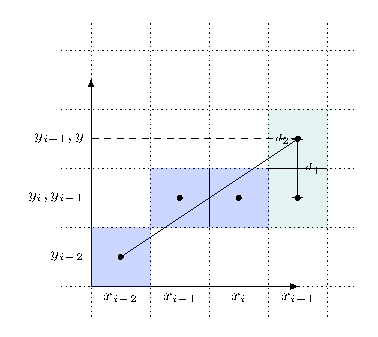
\includegraphics[width=\textwidth]{Chapter1/Bresenham/bresenham-stepwise/bresenham-third-step.pdf}
    \captionof{figure}{Bottom-Left Image}
\end{minipage}%
\hfill
\begin{minipage}[b]{0.48\textwidth} % Bottom-right image
%    \centering
    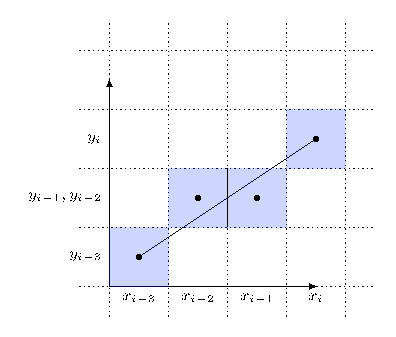
\includegraphics[width=\textwidth]{Chapter1/Bresenham/bresenham-stepwise/bresenham-fourth-step.pdf}
    \captionof{figure}{Bottom-Right Image}
\end{minipage}
\end{center}
\end{figure}

\subsection{Υλοποίηση αλγορίθμου για 1ο Οκταμόριο}

\subsubsection{Συνάρτηση ``φωτισμού" pixel}

Η παρακάτω συνάρτηση, παίρνει σαν είσοδο τις συντεταγμένες ενός σημείου στο επίπεδο, $\mathbb{R}^2$ και εκτυπώνει γράφημα με χρωματισμένο τετράγωνο πλευράς $1$ και κέντρο, το σημείο με τις συντεταγμένες της εισόδου:

\begin{lstlisting}[caption={Julia function to draw a rectangle}]
function draw_rectangle(x, y, color, test=true)
    # Define the coordinates of the rectangle vertices
    x_vertices = [x - 0.5, x + 0.5, x + 0.5, x - 0.5, x - 0.5]
    y_vertices = [y - 0.5, y - 0.5, y + 0.5, y + 0.5, y - 0.5]
    
    # Plot the rectangle
    if test    
        plot(x_vertices, y_vertices, aspect_ratio=:equal, 
             color=color, fill=true, legend=false, alpha=0.5)
        scatter!([x], [y], color=:red, aspect_ratio=:equal)
    else     
        plot!(x_vertices, y_vertices, aspect_ratio=:equal, 
              textwidth=2, color=color, fill=true, legend=false, alpha=0.7)
    end    
end
\end{lstlisting}

Οπότε, αν ο χρήστης εισάγει τις συνταταγμένες 2 σήμειων, έστω $P_1(x_1,y_1), P_2(x_2,y_2)$, τα οποία ανήκουν στο $1$ο οκταμόριο, τότε καλώντας παραπάνω αλγόριθμο, λαμβάνουμε τα κέντρα των pixel που σχεδιάζουν την ευθεία Bresenham που ενώνει τα $2$ σημεία.

\begin{example}
\end{example}


\begin{lstlisting}[caption={Bresenham Line Algorithm for 1st Octant}]
	function Bresenham_first_oct(x1, y1, x2, y2) 
	    dx = x2 - x1
	    dy = y2 - y1
	    x = x1
	    y = y1
	    c1 = 2 * dy
	    e = 2 * dy - dx
	    c2 = e - dx
	    
	    # Initialize L matrix with data points (x2-x1+1 points)
	    L = zeros(Int, 2, dx + 1)
	    
	    L[1, 1] = x #x coordinates in 1st row
	    L[2, 1] = y #2 coordinates in 2nd row
	
	    while x <= x2
	        L[1, x - x1 + 1] = x
	        L[2, x - x1 + 1] = y
	        
	        x += 1
	        if e < 0
	            e += c1
	        else
	            y += 1
	            e += c2
	        end
	    end
	    return [L[1,:], L[2,:]]
	end
\end{lstlisting}

\subsection{Σκιαγράφηση μεθόδου για σημεία εκτός 1ου οκταμορίου}

Αρκεί να εξετάσουμε τη συμπεριφορά της μεθόδου για τα οκταμόρια $1, 2, 3, 4$ (γιατί;)
 
Στην αρχική ιδέα του Bresenham παίζει σημαντικό ρόλο η σειρά που θα δώσουμε τα σημεία $P_1$ και $P_2$, Δηλαδή ποιο είναι η αρχή και ποιο το τέλος του τμήματος. Έτσι προκύπτουν 8 διαφορετικές περιπτώσεις. Αν, όμως, απλά θέλουμε να σχεδιάσουμε ένα ευθύγραμμο τμήμα, δεν μας ενδιαφέρει από ποια μεριά θα ξεκινήσουμε τον σχεδιασμό του. Συμφωνούμε να επιλέγουμε πάντα σαν αρχή το σημείο για την τετμημένη του οποίου ισχύει $y = min(y_1,y_2)$. Τότε, αντί για 8 περιπτώσεις, έχουμε μόνο 4, αφού τα οκταμόρια $5, 6, 7, 8$ ανάγονται σε $1, 2, 3, 4$ αντίστοιχα.

\begin{example}[Αναγωγή από 8ο οκταμόριο σε 4ο οκταμόριο]
	Έστω τα σημεία $P_1(2,-1), P_2(4,-3)$, τα οποία όπως είναι φανερό, ανήκουν στο $8$ο οκταμόριο.
\end{example}
%
%
\begin{figure}[h!]
  \begin{center}
	  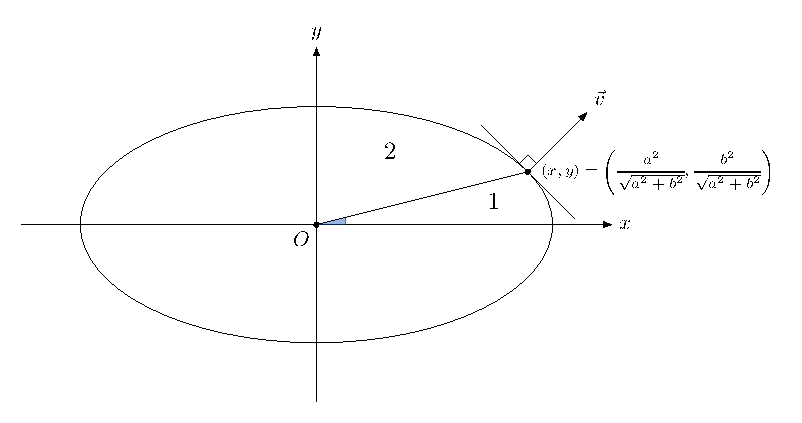
\includegraphics[scale=1]{Chapter1/Bresenham/axis-transformation/figure1.pdf}
  \end{center}
  \caption{Πρώτο βήμα αναγωγής 8ου τεταρτημορίου σε 4ο}
\end{figure}
%
%
\textbf{Βήμα 1:} Διαλέγω σαν αρχή το στοιχείο που έχει μικρότερη τεταγμένη, δηλαδή το $P_2$, και μετονομάζω: $P_1 \to P_2'\quad \text{και} \quad P_2 \to P_1'$.
%
%

\begin{minipage}{\textwidth}
	\begin{minipage}[b]{0.5\textwidth} % Top-left image
	    \centering
	    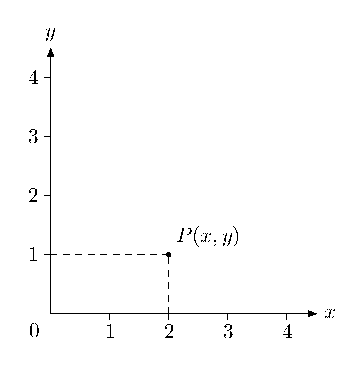
\includegraphics[width=\textwidth]{Chapter1/Bresenham/axis-transformation/figure2a.pdf}
%	    \captionof{figure}{Top-Left Image}
	\end{minipage}%
	\hfill
	\begin{minipage}[b]{0.5\textwidth} % Top-right image
	    \centering
	    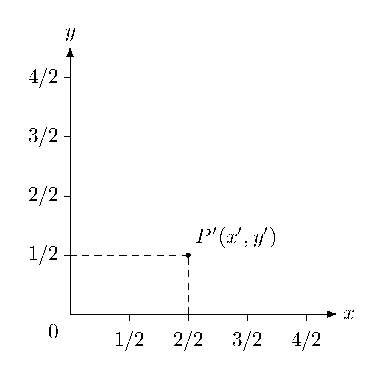
\includegraphics[width=\textwidth]{Chapter1/Bresenham/axis-transformation/figure2b.pdf}
	\end{minipage}
	\captionof{figure}{Επιλέγοντας αρχή των νέων αξόνων το σημείο με τη μικρότερη συντεταγμένη}
\end{minipage}
%
%
\textbf{Βήμα 2:} Παρατηρώ, φέρνοντας νέους νοητούς ορθοκανονικούς άξονες με αρχή το $P_1'$, ότι το ευθύγραμμό τμήμα που καλούμαι να σχεδιάσω σύμφωνα με τον αλγόριθμο του Bresenham ανήκει στο 4o Οκταμόριο.


\begin{minipage}{1\textwidth}
	\begin{minipage}[b]{0.48\textwidth} % Top-left image
	    \centering
	    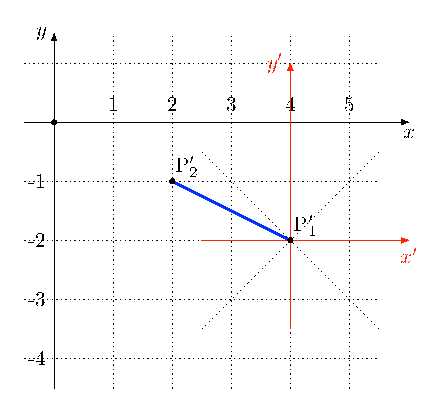
\includegraphics[width=\textwidth]{Chapter1/Bresenham/axis-transformation/figure3a.pdf}
%	    \captionof{figure}{Top-Left Image}
	\end{minipage}%
	\hfill
	\begin{minipage}[b]{0.48\textwidth} % Top-right image
	    \centering
	    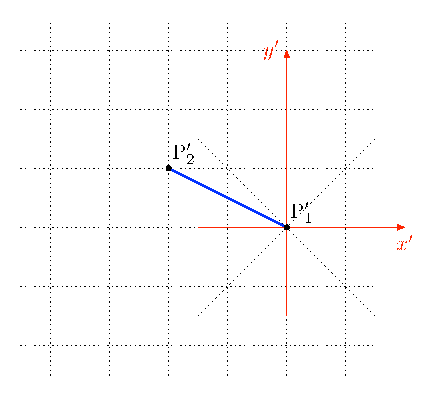
\includegraphics[width=\textwidth]{Chapter1/Bresenham/axis-transformation/figure3b.pdf}
	\end{minipage}
	\captionof{figure}{Επιλέγοντας αρχή των νέων αξόνων το σημείο με τη μικρότερη συντεταγμένη}
\end{minipage}

%% 2o oktamorio
\subsection{Αλγόριθμος του Bresenham για σημεία στο 2ο οκταμόριο}

Έστω $P_1(x_1,y_1), P_2(x_2,y_2)$, τα οποία ανήκουν στο $2$ο οκταμόριο. Ο σχεδιασμός της ευθείας του Bresenham στο $2$ο οκταμόριο γίνεται αν χρησιμοποιήσουμε στον αλγόριθμο του Bresenham τα συμμετρικά τους ως προς την $1$η διχοτόμο, δηλαδή τα σημεία $P_1' = (y_1, x_1)$ και $P_2' = (y_2, x_2)$. Τότε, εκμεταλλευόμενοι τη συμμετρία αυτή, αντί να φωτίζουμε το pixel $(x, y)$ που θα μας επιστρέφει ο αλγόριθμος εμείς φωτίζουμε το $(y, x)$. 

\begin{remark}
	Ο φωτισμός των συμμετρικών ως προν την 1η διχοτόμο pixel που θα προκύψουν από τον αλγόριθμο του Bresenham μπορεί να γίνει μία και καλή όταν περατωθεί ο αλγόριθμος. Αυτό μπορεί να συμβεί καθώς ο αλγόριθμος που έχουμε διατυπώσει επιστρέφει τα σημεία που πρέπει να φωτιστούν για να σχηματιστεί η επιθυμητή ευθεία. 
\end{remark}

\begin{minipage}{1\textwidth}
	\begin{minipage}[b]{0.48\textwidth} % Top-left image
	    \centering
	    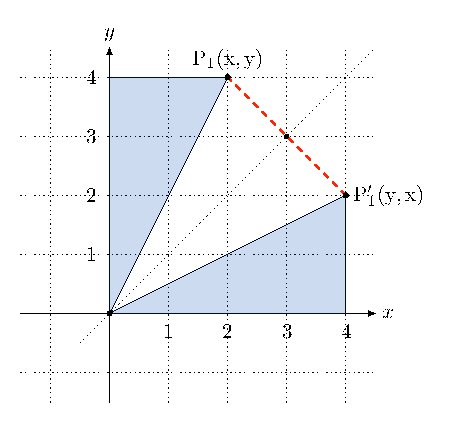
\includegraphics[width=\textwidth]{Chapter1/Bresenham/symmetries/symmetry-2nd.pdf}
%	    \captionof{figure}{Top-Left Image}
	\end{minipage}%
	\hfill
	\begin{minipage}[b]{0.48\textwidth} % Top-right image
	    \centering
	    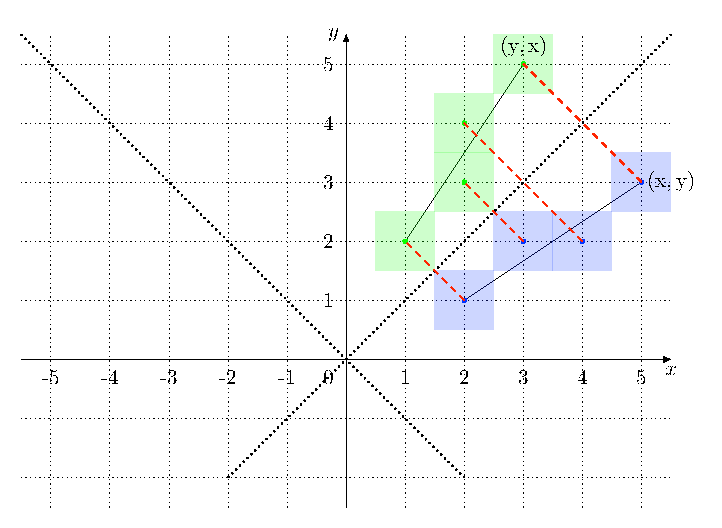
\includegraphics[width=\textwidth]{Chapter1/Bresenham/symmetries/bresenham-2nd.pdf}
	\end{minipage}
	\captionof{figure}{Συμμετρία μεταξύ 1ου και 2ου οκταμορίου που εκμεταλλεύομαστε για σηματισμό ευθείας σύμφωνα με αλγόριθμο του bresenham}
\end{minipage}

\begin{lstlisting}[caption={Bresenham Line Algorithm for 2nd Octant}]
function Bresenham_second_oct(x1, y1, x2, y2) 
	xPoints1, yPoints1 = Bresenham_first_oct(y1, x1, y2, x2)  
    for i in 1:xPoints1[end] - xPoints1[1]+1
        draw_rectangle(xPoints1[i], yPoints1[i], "blue", false)
		draw_rectangle(yPoints1[i], xPoints1[i], "green", false)
    end
endfunction    
\end{lstlisting}


%% 3o oktamorio
\subsection{Αλγόριθμος του Bresenham για σημεία στο 3ο οκταμόριο}

Έστω $P_1(x_1,y_1), P_2(x_2,y_2)$, τα οποία ανήκουν στο $3$ο οκταμόριο. Ο υπολογισμός των σημείων στο $3$ο οκταμόριο γίνεται αν θεωρήσουμε ότι στη θέση των $P_1$ και $P_2$, εισάγουμε τα σημεία $P_1' = (y_1, -x_1)$ και $P_2' = (y_2, -x_2)$. Τότε, αντί να φωτίζουμε το pixel $(x, y)$ που θα μας επιστρέφει ο αλγόριθμος εμείς φωτίζουμε το $(y, -x)$. Αυτό βέβαια, δεν είναι αναγκαίο να το κάνουμε σε κάθε βήμα του αλγορίθμου· μπορούμε να το κάνουμε μία και καλή, όταν περατωθεί ο αλγόριθμος.


\begin{minipage}{1\textwidth}
	\begin{minipage}[b]{0.48\textwidth} % Top-left image
	    \centering
	    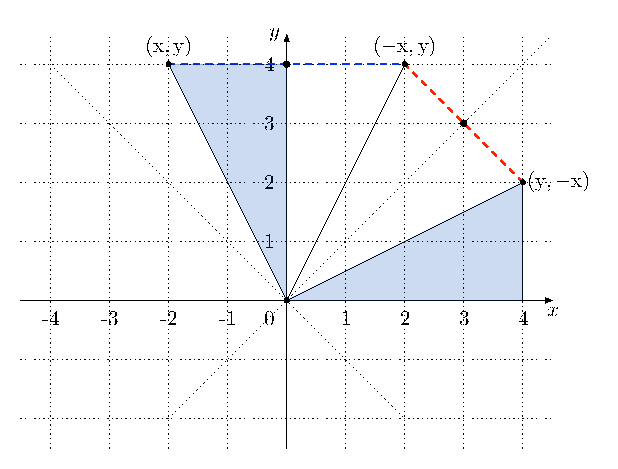
\includegraphics[width=\textwidth]{Chapter1/Bresenham/symmetries/symmetry-3rd.pdf}
%	    \captionof{figure}{Top-Left Image}
	\end{minipage}%
	\hfill
	\begin{minipage}[b]{0.48\textwidth} % Top-right image
	    \centering
	    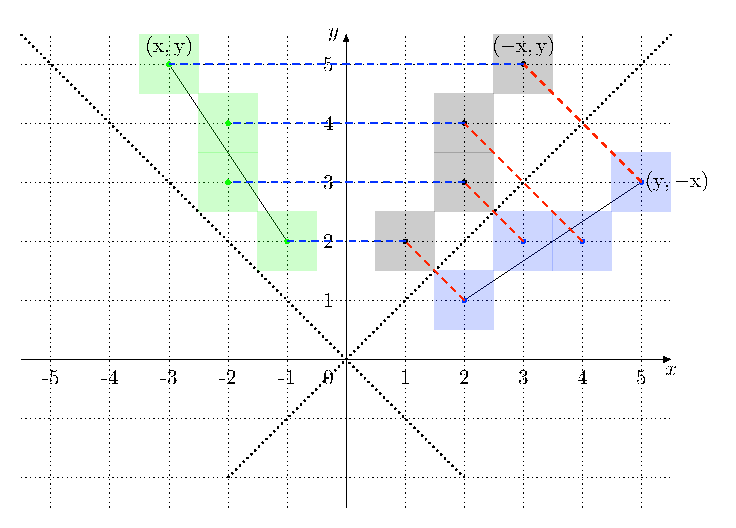
\includegraphics[width=\textwidth]{Chapter1/Bresenham/symmetries/bresenham-3rd.pdf}
	\end{minipage}
	\captionof{figure}{Συμμετρία μεταξύ 1ου και 2ου οκταμορίου που εκμεταλλεύομαστε για σηματισμό ευθείας σύμφωνα με αλγόριθμο του bresenham}
\end{minipage}

\begin{lstlisting}[caption={Bresenham Line Algorithm for 3rd Octant}]
function Bresenham_second_oct(x1, y1, x2, y2) 
	#(y1, -x1) and (y2, -x2) are the symmetric of (x1, y1) and (x2, y2) respectively in the 1st octant
	
	xPoints1, yPoints1 = Bresenham_first_oct(y1, -x1, y2, -x2)  
    for i in 1:xPoints1[end] - xPoints1[1]+1
        draw_rectangle(xPoints1[i], yPoints1[i], "blue", false)
		draw_rectangle(yPoints1[i], xPoints1[i], "gray", false)        
		draw_rectangle(-yPoints1[i], xPoints1[i], "green", false)
    end
endfunction    
\end{lstlisting}



%% 4o oktamorio
\subsection{Αλγόριθμος του Bresenham για σημεία στο 4ο οκταμόριο}

Έστω $P_1(x_1,y_1), P_2(x_2,y_2)$, τα οποία ανήκουν στο $4$ο οκταμόριο. Ο υπολογισμός των σημείων στο $4$ο οκταμόριο γίνεται αν θεωρήσουμε ότι στη θέση των $P_1$ και $P_2$, εισάγουμε τα σημεία $P_1' = (-x_1, y_1)$ και $P_2' = (-x_2, y_2)$ και αντί για να φωτίζουμε το pixel $(x, y)$ που θα μας επιστρέφει ο αλγόριθμος εμείς φωτίζουμε το $(-x, y)$. Αυτό βέβαια, δεν είναι αναγκαίο να το κάνουμε σε κάθε βήμα του αλγορίθμου· μπορούμε να το κάνουμε μία και καλή, όταν περατωθεί ο αλγόριθμος.


\begin{minipage}{1\textwidth}
	\begin{minipage}[b]{0.48\textwidth} % Top-left image
	    \centering
	    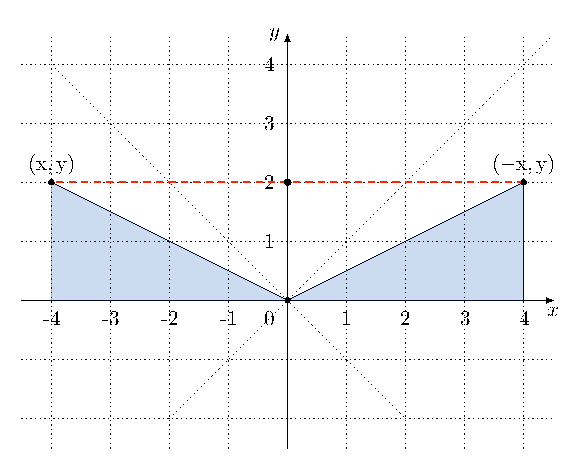
\includegraphics[width=\textwidth]{Chapter1/Bresenham/symmetries/symmetry-4th.pdf}
%	    \captionof{figure}{Top-Left Image}
	\end{minipage}%
	\hfill
	\begin{minipage}[b]{0.48\textwidth} % Top-right image
	    \centering
	    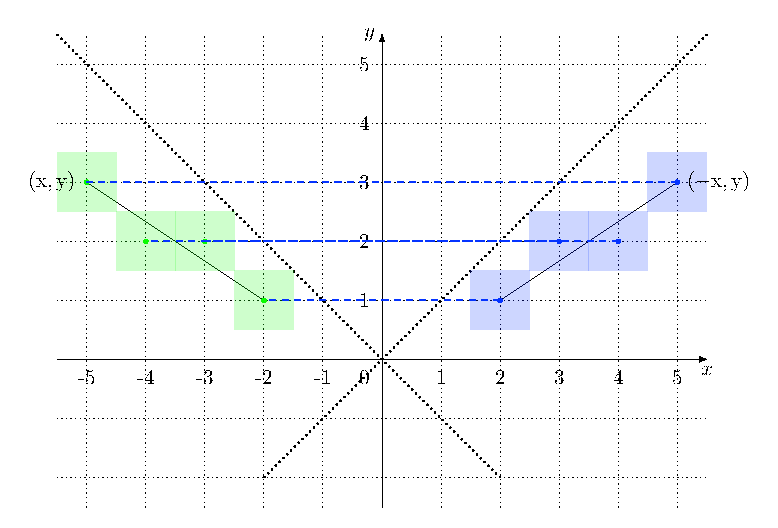
\includegraphics[width=\textwidth]{Chapter1/Bresenham/symmetries/bresenham-4th.pdf}
	\end{minipage}
	\captionof{figure}{Συμμετρία μεταξύ 1ου και 2ου οκταμορίου που εκμεταλλεύομαστε για σηματισμό ευθείας σύμφωνα με αλγόριθμο του Bresenham}
\end{minipage}

\begin{lstlisting}[caption={Bresenham Line Algorithm for 4th Octant}]
function Bresenham_second_oct(x1, y1, x2, y2) 
	#(-x1, y1) and (-x2, y2) are the symmetric of (x1, y1) and (x2, y2) respectively in the 1st octant
	
	xPoints1, yPoints1 = Bresenham_first_oct(-x1, y1, -x2, y2)  
    for i in 1:xPoints1[end] - xPoints1[1]+1
        draw_rectangle(xPoints1[i], yPoints1[i], "blue", false)
		draw_rectangle(-xPoints1[i], yPoints1[i], "green", false)        
    end
endfunction    
\end{lstlisting}

\subsection{Γενικός Αλγόριθμος Bresenham}
	Αν συνδυάσουμε όλα τα παραπάνω τότε προκύπτει ο παρακάτω αλγόριθμος που σχεδιάζει ευθεία που ενώνει δύο σημεία που παρίστανται στο επίπεδο σύμφωνα με τη λογική του αλγορίθμου του Bresenham.
	
	
\begin{lstlisting}[caption={General Bresenham Line Algorithm}]
function Bresenham_line(x1, y1, x2, y2)
	# Select starting point with the smallest y coordinate
    if y2 < y1
        x1, x2 = x2, x1
        y1, y2 = y2, y1
    end       
	# Find octants
    dx = x2 - x1
    dy = y2 - y1
    s = dy/dx
    if s <= 1 && s >= 0 # oct 1
        xPoints, yPoints = Bresenham_first_oct(x1, y1, x2, y2)  
    elseif s > 1 # oct 2
        xPoints, yPoints = Bresenham_first_oct(y1, x1, y2, x2) 
        
        xPoints, yPoints = yPoints, xPoints #from 1st octant, back to 2nd so i switch xPoints with yPoints

    elseif s < -1 # oct 3
        xPoints, yPoints = Bresenham_first_oct(y1, -x1, y2, -x2) 
        #from 1st octant, back to 3rd: 
            xPoints, yPoints = yPoints, xPoints #1. switch xPoints with yPoints to go to 2nd octant 
            
            xPoints, yPoints = -xPoints, yPoints #2. mirror with respect to new xPoints to go from 2nd to third

    else # oct 4
        xPoints, yPoints = Bresenham_first_oct(-x1, y1, -x2, y2)
        
        xPoints, yPoints = -xPoints, yPoints #from 1st octant, back to 4rd so: mirror with respect to xPoints 
    end
    
    # return [xPoints,yPoints]

    scatter(xPoints, yPoints, markersize=3, xlabel="x", ylabel="y", legend=false)
    # plot(xPoints, yPoints, xlabel="x", ylabel="y", legend=false, lc=:red) uncomment to add line

    for i in 1:size(xPoints,1)
        draw_rectangle(xPoints[i], yPoints[i], "blue", false)
    end

    plot!(title = "Bresenham line: ($x1,$y1) -> ($x2,$y2)", aspect_ratio=1)
    scatter!(xPoints, yPoints, markersize=3, xlabel="x", ylabel="y", legend=false)
    #savefig("giannis/outputs/line.png")   
endfunction
\end{lstlisting}	